\newcommand{\rsmpl}{\xleftarrow{\$}}

\newcommand{\alg}{\textsc{Alg}}

\newcommand{\ap}{\textsc{AccessPattern}}
\newtheorem{nonexample}[theorem]{Non-Example}


In an earlier lecture, we learned oblivious sorting, including bitonic sort with $\mathcal{O}(n \log^2 n)$ overhead~\cite{Batcher} , bucket oblivious sort~\cite{bucket} using oblivious random permutation to achieve $\mathcal{O}(n \log n (\log \log n)^2)$ overhead, 
and we showed that we can future eliminate the $(\log \log n)^2$ factor~\cite{domulticore, tianyao-sort}.
We will cover Hierarchical ORAM~\cite{10.1145/233551.233553} in today's lecture, which consists of a hierarchy of oblivious hash tables.
So, firstly, let's introduce oblivious hash table.

\section{Oblivious Hash Table}

\begin{definition}[Oblivious Hash Table]
    Consider a data array $A = \{ (k_i, v_i) | \bot \}_{i \in [N]}$, where $(k_i, v_i)$ is a real key-value pair element and $\bot$ is a filler. And it's guaranteed that all real elements have distinct keys. An oblivious hash table contains the following operations:
    \begin{itemize}
      \item Build($A$): Given a data array $A$, output a data structure.
      \item Lookup($k$): Given a key $k$, output $v$. If $k = \bot$ or $k \notin A$, $v = \bot$, otherwise $(k, v) \in A$.
    \end{itemize}
    $\forall A_0, op_0, A_1, op_1$ s.t. $|A_0| = |A_1|, |op_0| = |op_1|$ and both $(A_0, op_0)$ and $(A_1, op_1)$ satisfy the non-recurrent constraint, then the oblivious hash table requires: 
    $$\text{AccessPattern}(A_0, op_0) \approx \text{AccessPattern}(A_1, op_1)$$
    That is, for any data array and operation sequences of the same length, the access patterns in oblivious hash tables are indistinguishable as long as the same key is never looked up twice.
\end{definition}

Now let's introduce how to build an oblivious hash table.
We use the balls and bins hashing with $N$ elements (balls) and $N / Z$ bins, where $Z=\omega(\log N)$.
The expected number of elements in any fixed bin is $Z$. 
With Chernoff bound, the probability of any bin having more than $2Z$ elements is negligible.
Thus, we set the bin size to be $2Z$.

So now, we want to obliviously throw the balls into the bins without revealing which bin each ball goes to.
One way to randomly assign the element $(k, v)$ to a bin is to use a persudorandom function $PRF_{sk}(k)$, where the $sk$ is the secret key held by the ORAM client and the PRF output range is $[N/Z]$, indicating the bin index.
To do this obliviously, we can use the butterfly network to route the elements to their respective bins, which is similar to the oblivious random permutation.
So, everytime the clients lookup a fresh element, the ORAM servers will see they are accessing a random bin. In case if it's a filler element, the client will just lookup a random bin.

\textbf{Analysis.} Building an oblivious hash table involves routing elements to random bins. 
Recall that in oblivious random permutation, we can accomplish this with $\mathcal{O}(N \log N)$ overhead~\cite{domulticore, tianyao-sort}. 
For every lookup, the cost is the bin size, which is $Z = \omega(\log N)$.
Different from static hashing that has constant cost for each lookup, oblivious hash tables have a bit higher overhead.

\section{Hierarchical ORAM}

So now with this oblivious hash table, we can construct a Hierarchical ORAM.
In Hierarchical ORAM, we have a hierarchy of exponentially growing oblivious hash tables as shown in Figure~\ref{fig:oram}.
Each level of the hierarchy has a different capability, and the capability grows exponentially with the level.
The $i$-th level's capability is $2^i$.
The root level has the largest capability $2^L$, where $L = \lceil \log N \rceil$, and the leaf level has the smallest capability $1$.
Additionally, every level has a label, either \textbf{available} (\textbf{empty}) or \textbf{full}.

\begin{figure}[!h]
  \centering
  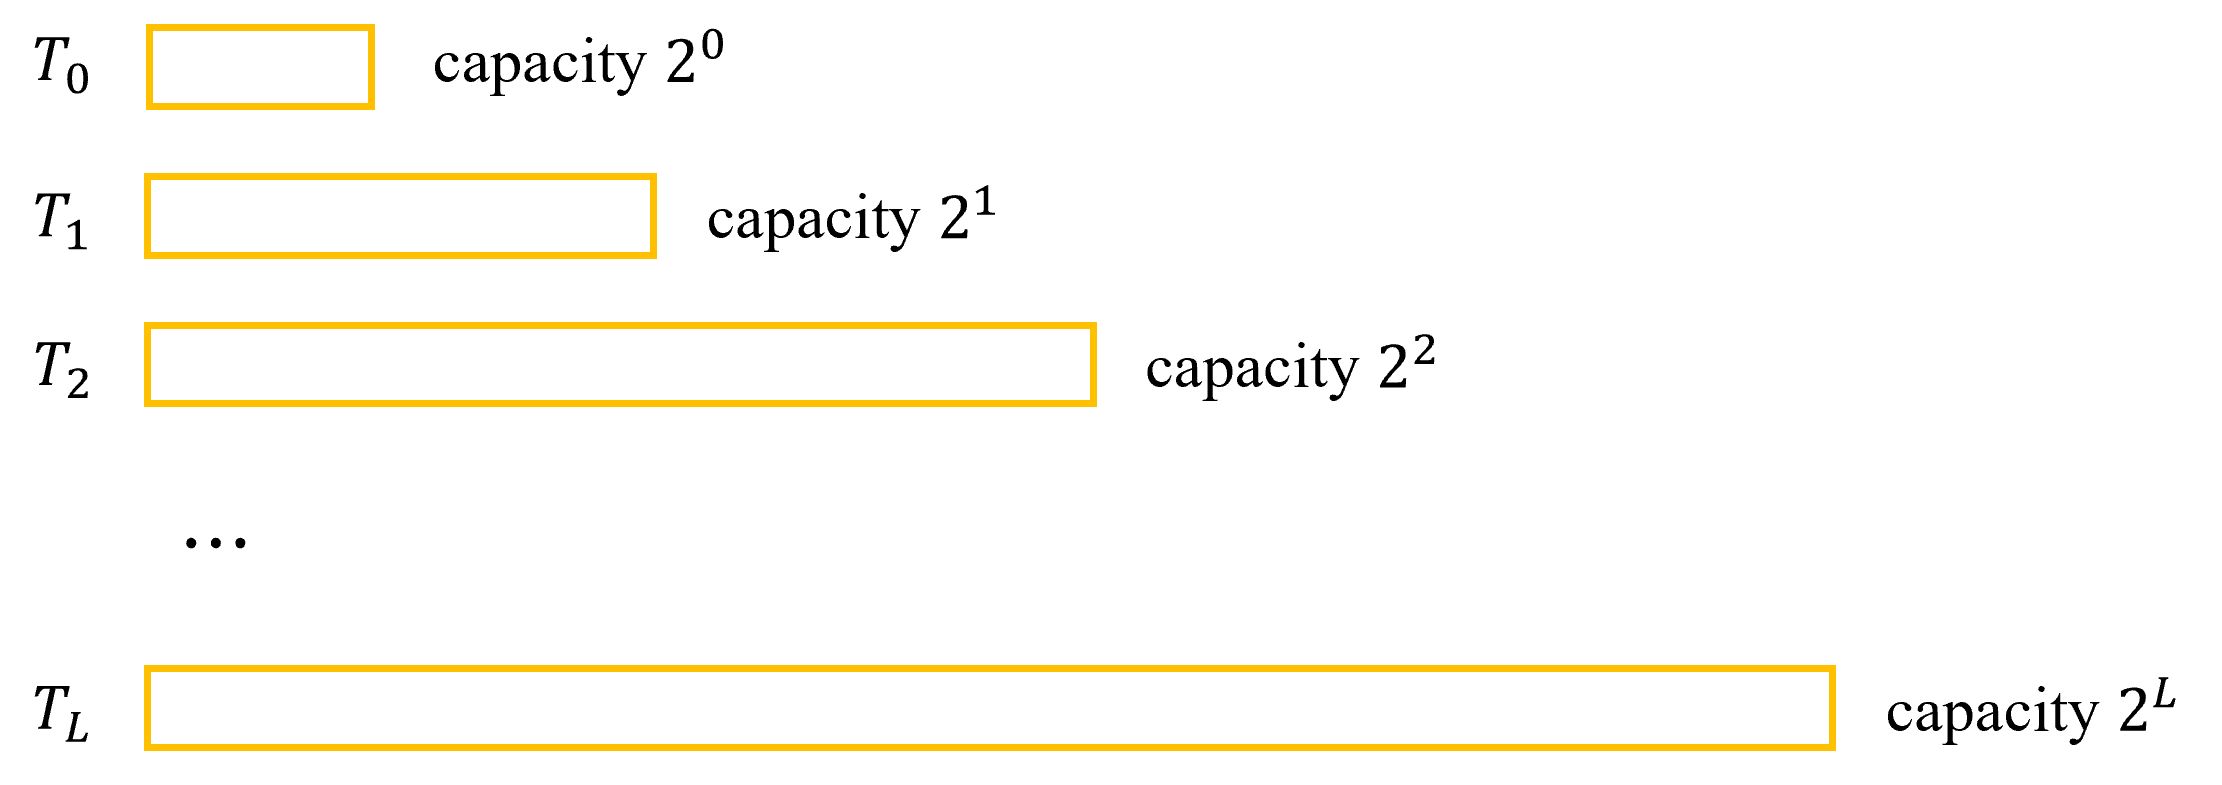
\includegraphics[width=0.8\textwidth]{fig1.png}
  \caption{Hierarchical ORAM}
  \label{fig:oram}
\end{figure}

Now let's consider two operations, \texttt{Read}(\texttt{addr}) and \texttt{Write}(\texttt{addr}, \texttt{data}).
Before we dive into the detailed algorithm, let's first introduce the high-level idea of how to perform these operations.

If we want to lookup some element, we will start from the smallest level.
Since every level is either empty or full. If it's full, lookup in that hash table for the element.
There are two outcomes: either we find the element, or we don't find the element.
If we find the element, for all future levels, we just lookup filler and perform a fake operation.
Similar to the tree-based ORAM, we will also need to relocate the retrived element.
So in Hierarchical ORAM, we will put the retrived element to the smallest level if this level is empty.
If this level is not empty, we will need to merge the retrived element with the existing element in this level and put the merged element to the next level. 
Otherwise, if this level is still not empty, merge them again and put them to the next level, until we find the empty level to put the merged element.

\textbf{Algorithm.} The detailed algorithm is shown in Algorithm~\ref{alg:oram}. The algorithm starts by initiating a binary variable \texttt{found} to \texttt{false}.
Then, for each level, we check if the element is in the hash table. 
If we find the element, we set \texttt{found} to \texttt{true} and store the element in $\texttt{data}^*$.
If the element is already found, we just lookup filler in the hash table for the rest of the levels to prevent leakage in the access patterns.
After we go through all levels, the fetched element is in $\texttt{data}^*$.

In the following we will do the relocate operation.
If the operation $\texttt{op}$ is \texttt{read}, we will need to relocate the retrived element $T^\phi = \{(\texttt{addr}, \texttt{data}^*)\}$.
Otherwise, if the operation $\texttt{op}$ is \texttt{write}, we will need to relocate the new element $T^\phi = \{(\texttt{addr}, \texttt{data})\}$.
Let $l$ be the smallest level such that $T_l$ is empty, if all levels are full, let $l = L$.
Let $S$ be the set of elements to relocate, which is the union of the new element and all the elements in the hash tables from level $0$ to level $l-1$.
If all levels are full, let $S$ be the union of all the elements and the new element $T^\phi$.
Then we build the hash table at level $l$ with the set $S$.
The build step is the same as the oblivious hash table, which is to throw the elements into the bins obliviously.
After the build step, we mark the level $l$ as full and the levels $0$ to $l-1$ as empty.

Note that if the oblivious hash table doesn't remove the element we just looked up, there might be duplicate elements in the set $S$ and we will need to suppress the duplicate elements.
The elements in the smaller level is always fresher than the elements in the larger level, so we can just keep the fresher element and remove the older one.
We use the oblivious sorting to do the \texttt{SuppressDup}, which simply sorts the elements by key and by freshness and removes the duplicate elements using a linear scan.


\begin{algorithm}[h]
  \SetAlgorithmName{Algorithm}{algorithmautorefname}{list of algorithms name}
  \caption{\textsc{Hierarchical ORAM}}
  \label{alg:oram}
 
 \KwIn{$\texttt{addr}$, an address to lookup in the hash tables; $\texttt{op}$, the operation $\texttt{write}$ or $\texttt{read}$; $\texttt{data}$, the data to write.}
 \KwOut{$data^*$, the lookup result, if $\texttt{op} = \texttt{read}$.}
 $\texttt{found} \leftarrow false$\;
 \For{$l \leftarrow 0$ \KwTo $L$}{
   \If{not $\texttt{found}$}{
     $\texttt{fetched} \leftarrow T_l.lookup(\texttt{addr})$\;
     \If{$\texttt{fetched} \neq \bot$}{
        $\texttt{found} \leftarrow true$\;
        $data^* \leftarrow \texttt{fetched}$\;
     }
   }
   \Else{
      $T_l.lookup(\bot)$
   }
 }
 \If{$\texttt{op} = \texttt{read}$}{
  Let $T^{\phi} \leftarrow \{ (\texttt{addr}, \texttt{data}^*) \}$\;
 }
 \ElseIf{$\texttt{op} = \texttt{write}$}{
  Let $T^{\phi} \leftarrow \{ (\texttt{addr}, \texttt{data}) \}$\;
 }
 Let $l$ be the smallest level such that $T_l$ is empty, if all levels are full, let $l = L$\;
 Let $S \leftarrow T^\phi \cup T_0 \cup \cdots \cup T_{l-1}$\;
 If all levels are full, let $S \leftarrow S \cup T_L$\;
 $T_l.Build(\texttt{SuppressDup}(S))$\;
 Mark $T_l$ as full\;
 Mark $T_0, \cdots, T_{l-1}$ as empty\;
 \If{$\texttt{op} = \texttt{read}$}{
  \Return{$\texttt{data}^*$}\;
 }
 \end{algorithm}

\textbf{Analysis.} Now let's analyze the overhead of Hierarchical ORAM. There are two sources of the overhead: the lookup phase, and the rebuild phase.
The lookup cost is $L \times Z$, the number of levels $L$ times the lookup cost of at each level, which is at most $Z$. Recall $Z = \log N \cdot \alpha(N)$, where $\alpha(N)$ is the superconstant function. Thus the lookup cost is $\mathcal{O}(\log^2 N \cdot \alpha(N))$.

For rebuild cost, a level of size $2^i$ is rebuilt every $2^i$ steps.
So to rebuild a level of size $2^i$, the cost is $2^i \cdot \log 2^i$ (see the analysis of the oblivious hash table).
By amortizing the cost to each step, every level has a cost $\leq \log N$.
Thus, the rebuild cost is $\mathcal{O}(\log^2 N)$.
Note that the original Goldreich-Ostrovsky construction~\cite{10.1145/233551.233553} has a cost of $\mathcal{O}(\log^3 N)$, because that they throw $N$ balls into $N$ bins, instead of $N/Z$ bins.